\documentclass{article}
\usepackage{amsmath}
\usepackage{hyperref}
\usepackage{graphicx}
\usepackage{adjustbox}
\newcommand{\tabincell}[2]{\begin{tabular}{@{}#1@{}}#2\end{tabular}}

\begin{document}
\begin{titlepage}
\title{EE 239AS \\Special Topics in Signals and Systems\\Project 4\\Popularity Prediction on Twitter\\Winter 2016} 
\author{Liqiang YU, Kaiming WANG and Jun FENG\\
904592975, 504592374, 304588434} 
\date{03-18-2016}
\end{titlepage}

\maketitle
\newpage
\tableofcontents
\newpage

\section{Introduction}
The Twitter website, as the most famous social network, is a good source to predict future popularity of a subject or event. In this project, we analyzed the data from twitter crawled during the period of 2015 superbowl, from two weeks before the game to one week after the game. We trained different regression models for tweets with different hashtags to predict the number of tweets in the next hour. We included features both from the tutorial and our own design. And we used the test set to evaluate our model's prediction results. Finally, we came up with a new idea based on the rich data from the twitter, that is try to describe the emotion change of fans from both teams during and after the game, based on the contents from their tweets.\\
\\
The report is organized as follows : in section \ref{sec:data_analysis}, we did a quick scan through the file and got some statistics information about the data....
\section{Data Analysis}\label{sec:data_analysis}
We have six hashtags for training : \#gohawks, \#gopatriots, \#nfl, \#patriots, \#sb49, \#superbowl.
The data information is shown in table \ref{tb:data_information}. The distribution for \#superbowl and \#nfl are shown in figure \ref{fig:sp_hist} and \ref{fig:nfl_hist}. We only consider the time period of interest, which is two weeks before Feb 1st, 2015 and one week after it. From the histograms we can see that both hashtags concentrated during the game time, especially for \#SuperBowl. For \#NFL, there was another peak during the last weekend before the superbowl final game, which showed that people would like to talk about the NFL game during weekends.
\begin{table}[hbp]
\caption{The data information for each hashtag}
\begin{adjustbox}{center}

\label{tb:data_information}
\begin{tabular}{|c|c|c|c|c|c|c|}
\hline
& gohawks & gopatriots & nfl &patriots & sb49 & superbowl\\
\hline
\tabincell{c}{Average number of \\tweets per hour} & 380.84 & 53.43 & 515.98 & 975.52 & 1647.31 & 2692.14\\
\hline
\tabincell{c}{Average number of \\follower per users}& 1544.97 & 1298.82 & 4289.75 & 1650.32 & 2235.16 & 3591.60\\
\hline
\tabincell{c}{Average number of \\retweets per tweet}& 2.01& 1.40 & 1.54 & 1.78 & 2.51 & 2.39\\
\hline
\end{tabular}
\end{adjustbox}
\end{table}

\begin{figure}[htbp]
\centering
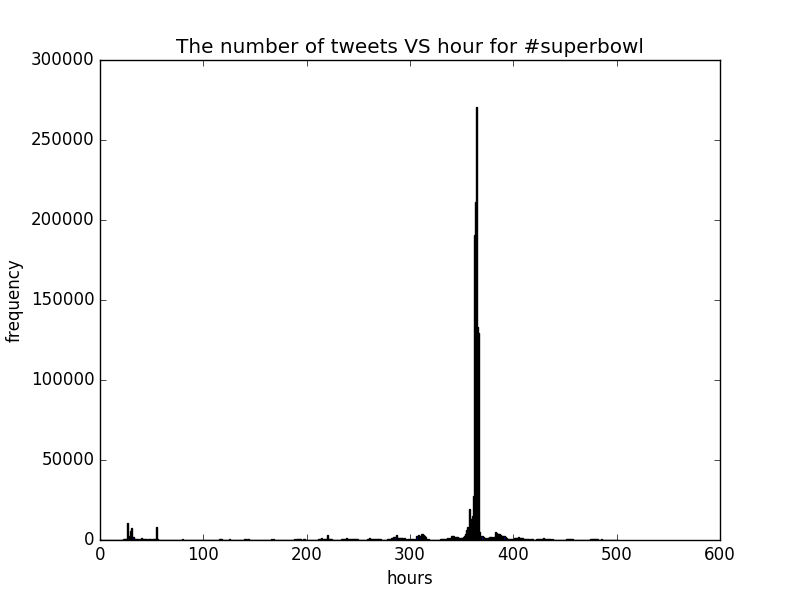
\includegraphics[width=.6\textwidth]{sp_hist.png}
\caption{The histogram for \#SuperBowl}
\label{fig:sp_hist}
\end{figure}
\begin{figure}[htbp]
\centering
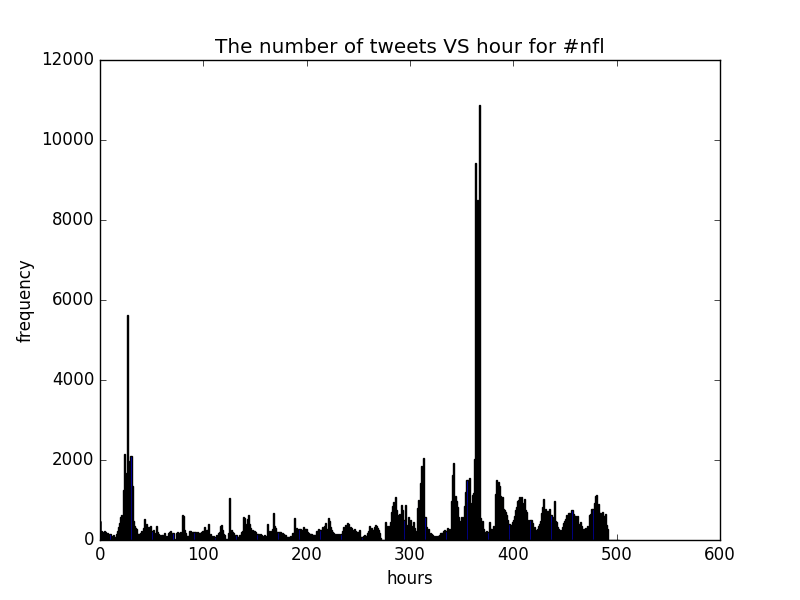
\includegraphics[width=.6\textwidth]{nfl_hist.png}
\caption{The histogram for \#NFL}
\label{fig:nfl_hist}
\end{figure}
\section{Linear regression model}
In this section, we use linear regression model with five required features including number of tweets, total number of retweets, sum of the number of followers of the users posting the hashtag, maximum number of followers of the users posting the hashtag, and time of the day. About the last feature i.e. time of the day, we try to binarize this feature. According to the suggestion, we use one-hour window to predict tweet number of next hour from the previous one. \\
\\
P-value can tell us the accuracy while t-test can be used to note the significance of each feature. The result is in table \ref{tb:p21} and table \ref{tb:p22}.
\begin{table}
\caption{T-test of Different Hashtag}
\begin{adjustbox}{center}
\label{tb:p21}
\begin{tabular}{|l||c|c|c|c|c|}
\hline
Hashtag/feature & \tabincell{c}{Number of\\ Tweets}& \tabincell{c}{Total Number of\\ Retweets} & \tabincell{c}{Sum of Number of \\Followers of\\ the Users} & \tabincell{c}{Maximum Number of\\ Followers of\\  Users} & \tabincell{c}{Time of \\the Day}\\
\hline
gohawks&7.007&-2.900&-1.835&0.052&2.471\\
gopatriots&6.598&-2.912&-0.524&-0.462&2.264\\
nfl&6.506&-3.020&-0.386&0.524&2.152\\
patriots&14.968&-8.203&2.097&0.521&1.859\\
sb49&11.600&-4.032&3.221&2.243&-0.366\\
superbowl&8.992&-2.426&-1.116&1.912&-0.327\\
\hline
\end{tabular}
\end{adjustbox}
\end{table}

\begin{table}
\caption{P-value of Different Hashtag}
\begin{adjustbox}{center}
\label{tb:p22}
\begin{tabular}{|l||c|c|c|c|c|}
\hline
Hashtag/feature & \tabincell{c}{Number of\\ Tweets}& \tabincell{c}{Total Number of\\ Retweets} & \tabincell{c}{Sum of Number of \\Followers of\\ the Users} & \tabincell{c}{Maximum Number of\\ Followers of\\  Users} & \tabincell{c}{Time of \\the Day}\\
\hline
gohawks&0.000&0.004&0.067&0.959&0.014\\
gopatriots&0.000&0.004&0.601&0.644&0.024\\
nfl&0.000&0.003&0.700&0.600&0.032\\
patriots&0.000&0.000&0.036&0.602&0.064\\
sb49&0.000&0.000&0.001&0.025&0.714\\
superbowl&0.000&0.016&0.265&0.056&0.744\\
\hline
\end{tabular}
\end{adjustbox}
\end{table}

\section{Cross Validation and Time Period}
In this section, Firstly, we apply cross-validation to section 3. We divide set of \emph{(features,predictant)} into 10 parts. Each time, we fit our model with 9 parts and predict the number of tweets of remaining parts. We use average prediction error $|N_{predicted}-N_{real}|$ over all the samples in the remaining part to reflect the perfomance, the result is in table \ref{tb:p41}. We use both linear regression and polynomial regression, we may find that linear regression performs a bit better than polynomial regression.

\begin{table}
\caption{Average Prediction Error over Different Hashtags}
\begin{adjustbox}{center}
\label{tb:p41}
\begin{tabular}{|l||c|c|}
\hline
Hashtag & \tabincell{c}{Average Prediction Error\\(Linear regression)}&\tabincell{c}{Average Prediction Error\\(Polynomial regression)}\\
\hline
gohawks&244.911047&234.497215\\
gopatriots&246.475136&288.613566\\
nfl&404.397690&484.162998\\
patriots&852.457160&1317.653672\\
sb49&1250.245770&2259.266121\\
superbowl&2835.748989&3554.870260\\
\hline
\end{tabular}
\end{adjustbox}
\end{table}

From section 1, we can find that patterm is totally different among different period. So, we should divide the datasets into different period. In this project, we divide them into three periods according to first post time of tweets:

\begin{itemize}
        \item From 2015/01/16, 12:00:00 to 2015/02/01, 07:59:59 
        \item From 2015/02/01, 08:00:00 to 2015/02/01, 19:59:59 
        \item From 2015/02/01, 20:00:00 to 2015/02/07, 02:59:59 
      \end{itemize}

Then, we conduct 10-fold cross-validation in different period, in period 1 and period 3, we use polynomial regression model while in period 2, we still use linear regression model. The averge prediction error over different hashtags and peroids is in table \ref{tb:p42}. We may find that when in peroid 2, the performance of linear regression is near polynomial regression while in period 1 and peroid 2, linear regression performs much better than polynomial regression.


\begin{table}
\caption{Average Prediction Error over Different Hashtags and Periods}
\begin{adjustbox}{center}
\label{tb:p42}
\begin{tabular}{|l||c|c|c|c|c|c|c|}
\hline
 &  \tabincell{c}{Period 1\\(Linear)} & \tabincell{c}{ Period 1\\(Polynomial)} &  \tabincell{c}{Period 2\\(Linear)} &  \tabincell{c}{Period 2\\(Polynomial)} &  \tabincell{c}{Period 3\\(Linear)}&  \tabincell{c}{Period 3\\(Polynomial)}\\
\hline
gohawks&250.357506&358.964101&2349.263964&6797.216256&17.785470&21.548620\\
gopatriots&254.876108&382.702084&2377.095233&4262.882541&18.716673&33.497539\\
nfl&371.097217&1123.011263&3733.257332&14867.083123&114.001099&119.469134\\
patriots&474.265800&584.006864&15480.570477&20366.797150&157.526328&179.914494\\
sb49&552.755564&666.017315&35125.435713&74726.211367&247.370058&323.475495\\
superbowl&821.552995&930.019195&79503.117523&253415.804881&380.846079&463.248204\\
\hline
\end{tabular}
\end{adjustbox}
\end{table}

\section{Make prediction}
From the previous section, since we have 6 hashtags and 3 peroids, totally we have 18 models to make prediction. In this section, 10 test data has been given, after skimming over the data, we can get their peroids and hashtags. Then we can use the suitable models in last model to get the best prediction. The result of prediction is in table \ref{tb:p51}. We still contract two regression model. Since linear regression cannot produce resonable prediction in Period 2, we recognize polynomial regression as final result in Period 2 while we will use linear regression result in Peroid 1 and Peroid 3.

\begin{table}
\caption{Prediction of Number of Tweets for the Next Hour}
\begin{adjustbox}{center}
\label{tb:p51}
\begin{tabular}{|l||c|c|c|c|c|}
\hline
Testfile & Hashtag & Period  & Polynomial Regresssion& Linear Prediction \\
\hline
$sample1_period1.txt$&superbowl&Period 1&121&$-1.26\times 10^7$\\
$sample2_period2.txt$&superbowl&Period 2&203428&133499\\
$sample3_period3.txt$&superbowl&Period 3&676&$3.1\times 10^9$\\
$sample4_period1.txt$&gohawks&Period 1&248&$-3.26\times 10^8$\\
$sample5_period1.txt$&gohawks&Period 1&1240&$-1.25\times 10^8$\\
$sample6_period2.txt$&gohawks&Period 2&$-1.6\times 10^7$&27675 \\
$sample7_period3.txt$&gohawks&Period 3&33&723352\\
$sample8_period1.txt$&nfl&Period 1&17&-786142\\
$sample9_period2.txt$&nfl&Period 2&19622&5428\\
$sample10_period3.txt$&nfl&Period 3&101&1581925\\
\hline
\end{tabular}
\end{adjustbox}
\end{table}

\section{Description of the emotion change : Sentiment Analysis}
\subsection{Problem Statement}
When we get access to millions of twitter contents, what we are often interested in is what did the users say and what were their emotions at that time. This leads to the sentiment analysis and can be beneficial for lots of areas. For instance, during the president election campaign, the candidates want to know what the people's reactions are towards their recent lecture or debate, which gives them instructions on how to improve it in the future.\\
\\
Therefore, we tried to detect the emotion changes from fans of both teams during and after the final game with the tweet data we have. That is, we want to know whether we can detect more happiness from tweets of patriots fans and more sadness from fans of hawks.
\subsection{Data Preprocessing}
We used the 'tweet' metadata in json files, which represents the contents of that tweet. However some preprocessing steps need to be done before making the sentiment analysis.The steps include:\\
\begin{enumerate}
\item Tokenize the tweet text, which includes making all letters lowercase, getting rid of stop words and punctuations, and tokenizing the text with regular expressions which match common words, hashtags, urls, user mentions and simple emotion symbols like ":)".
\item Calculate the term frequency for each term appeared in the tweet contents.
\item Calculate the term co-occurences for each term appeared in the tweet contents.
\end{enumerate}
\subsection{Pointwise Mutual Information}
In this project, we define the Semantic Orientation(SO) of a word as the difference between its associations with positive and negative words. In practice, we want to calculate how close a word is with terms like \emph{good} and \emph{bad}. The chosen measure of closeness is Pointwise Mutual Information(PMI).\\
\begin{equation*}
PMI(t_1, t_2) = log\left( \frac{P(t_1\cap t_2)}{P(t_1)*P(t_2)}\right) 
\end{equation*} 
\\
Then the SO of a word is calculated against positive and negative terms. Let's define $V^+$ a set of positive words and $V^-$ a set of negative words, the SO of a term is defined as 
\begin{equation*}
SO(t) = \sum_{t'\in V^+}PMI(t, t')-\sum_{t'\in V^-}PMI(t, t')
\end{equation*}
We define the Document Frequency(DF) of a term as the number of documents where the term occurs, so the probablities are defined as:
\begin{equation*}
\begin{split}
&P(t) =\frac{DF(t)}{|D|}\\
&P(t_1\cap t_2) = \frac{DF(t1\cap t2)}{|D|}
\end{split}
\end{equation*}
\subsection{Results and Discussions}
We choose to use \#gohawks and \#patriots as the support hashtag for two teams because the amount of data in \#gopatriots is too small. We split the data into one hour period and only consider the 24 hours around the game. We plot the semantic orientation every hour for the twitter contents from two teams fans and make the comparison. \\
\\
The results are shown in figure \ref{fig:emotion24}. From the figure we can see that at first seahawks fans are more confident than patriots fans, however there was a turning point at around  6:30pm, which is 3 hour after the game start. When we enlarge that area and show it in figure \ref{fig:emotion6}, we can see that after that turning point patriots fans are much happier than hawks fans. After referring it to the game facts, we think it makes sense because it describes a story of bouncing back from behind and win the championship. \\
\\
The table \ref{tb:game} shows the game facts. From the game facts, we can see that at 190 minutes, which is nearly 3 hours after the game start, the hawks lead the patriots by 24:14, however after that the hawks got no point anymore and the patriots turned back and won the superbowl. Therefore it explained why hawks fans started to feel unhappy at the time 3 hours after the game start and why patriots felt happy.
\begin{figure}[htbp]
\centering
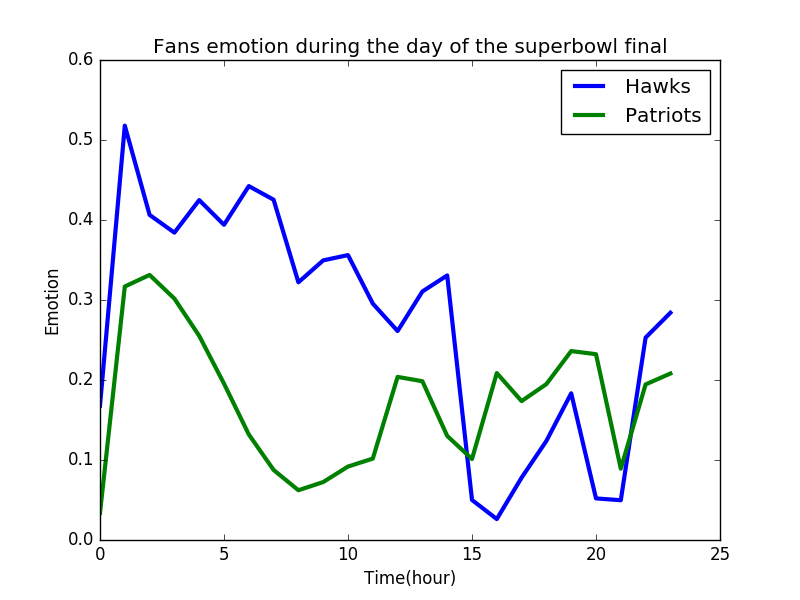
\includegraphics[width=.6\textwidth]{emotion24.png}
\caption{The emotion change during 24 hours}
\label{fig:emotion24}
\end{figure}

\begin{figure}[htbp]
\centering
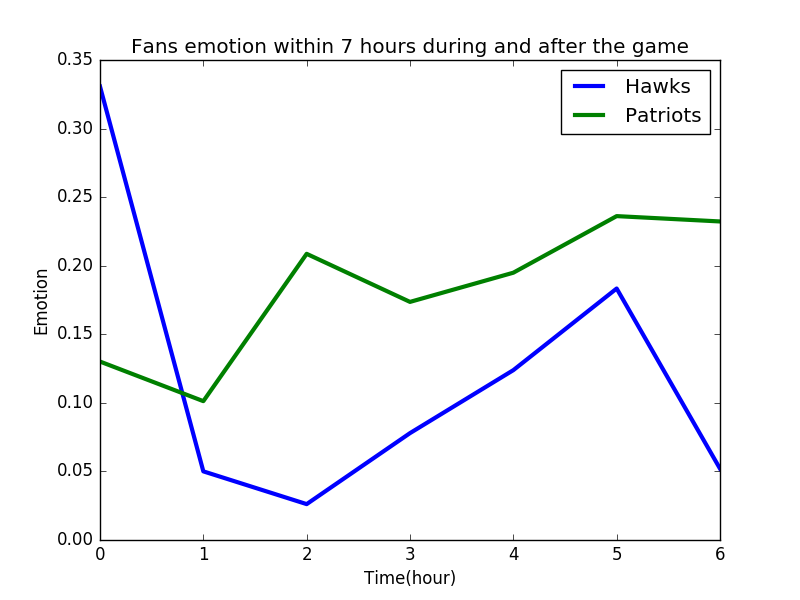
\includegraphics[width=.6\textwidth]{emotion6.png}
\caption{The emotion change from 2 hours to 8 hours after the game start  }
\label{fig:emotion6}
\end{figure}

\begin{table}[hbp]
\caption{Game facts for 2015 superbowl}
\begin{center}
\label{tb:game}
\begin{tabular}{|c|c|}
\hline
Minutes after the game start & Scores(Patriots : Hawks)\\
\hline
88&7:0\\
\hline
105&7:7\\
\hline
120&14:7\\
\hline
130&14:14\\
\hline
175&14:17\\
\hline
190&14:24\\
\hline
227&21:24\\
\hline
243&28:24\\
\hline
END&28:24\\
\hline
\end{tabular}
\end{center}
\end{table}
\end{document}
